%!TEX root = /Users/markelikalderon/Documents/Git/formwithoutmatter/aristotle.tex
\chapter{The Eye} % (fold)
\label{cha:the_eye}

\section{The Soul of the Eye} % (fold)
\label{sec:the_soul_of_the_eye}

Sight, Aristotle tells us, is the soul of the eye, or would be if it were an animal. This claim is made in the context of explaining what the soul of an animal is, and Aristotle proceeds by analogy with artifacts and parts of animals:
\begin{quote}
	Suppose that a tool, e.g. an axe, were a natural body, then being an axe would have been its essence, and so its soul; if this disappeared from it, it would have ceased to be an axe, except in name. As it is, it is an axe; for it is not of a body of that sort that what it is to be, i.e. its account, is a soul, but of a natural body of a particular kind, viz. one having in itself the power of setting itself in movement and arresting itself. Next, apply this doctrine in the case of the parts of the living body. Suppose that the eye were an animal—sight would have been its soul, for sight is the substance of the eye which corresponds to the account, the eye being merely the matter of seeing; when seeing is removed the eye is no longer an eye, except in name—no more than the eye of a statue or of a painted figure. (\emph{De Anima} \textsc{ii}.1 412\( ^{b} \)12--22)
\end{quote}

If an axe were a natural body, then what it is to be an axe would be both essential to the axe and its soul. If what it is to be an axe were somehow removed from a thing, then it would cease to be an axe. For a thing to have what it takes to be an axe is for that thing to possess a capacity for motion and rest characteristic of axes. Specifically, the thing must possess the capacity to cut in the manner of axes. Thus should a thing lose its capacity to cut, or to cut in that manner, it would cease to be an axe. It would be an axe in name only. The capacity to cut in the manner of axes is both the form and substance of an axe. If the capacity to cut in that manner is the form of an axe, then the material parts of the axe---the wooden shaft, the bronze head---constitute its matter. 

In the quoted passage, Aristotle notes an important limitation of the analogy. ``As it is, is an axe.'' That is to say, an axe is not, in fact, a natural body but is, rather, an artifact. Unlike a natural body, such as a living being, an axe does not contain within itself the power of motion and rest. An axe has the capacity to cut because of the use we make of it. The essential form and substance of an axe is not its soul. A living being is a natural body with a soul. But an axe, being an artifact, is not a natural body, and hence not a living being, and so lacks a soul.

Aristotle's account of the soul of an axe is the model for his account of the soul of an eye. If an eye were an animal, then what it is to be an eye would be both essential to the eye and its soul. If what it is to be an eye were somehow removed from a thing, then it would cease to be an eye. For a thing to have what it takes to be an eye is for that thing to possess the capacity for sight. Thus should a thing lose this capacity, it would cease to be an eye. It would be an eye in name only. A thing that lacks the capacity to see is like the eye of a statue, such as the drooping eye of King Seuthes \textsc{iii} in the 4th century \textsc{bc} Thracian bronze portrait, the trace, perhaps of an old battle wound (see figure~\ref{fig:seuthesiii}). The portrait is remarkably naturalistic, and the King's gaze is arresting. The artist used glass paste of different colors to distinguish the white of the eye, the pupil, and the iris, and thin copper wire for the eyelashes. Despite the striking naturalism and the intensity of the King's gaze, the drooping eye is, nonetheless, no real eye. Despite the naturalism and psychological expression achieved by the Thracian masterpiece, the colored glass paste, being opaque, lacks the capacity to see. The capacity to see is the form and substance of an eye. If the capacity to see is the form of the eye, then the material parts of the eye---the membrane, the interior water---constitute its matter.

\begin{figure}[htbp]
	\centering
		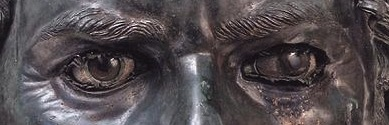
\includegraphics[scale=1]{graphics/seuthesiii.jpg}
	\caption{Detail of 4th century \textsc{bc} Thracian bronze portrait of King Seuthes \textsc{iii}}
	\label{fig:seuthesiii}
\end{figure}

If we suppose the eye to be an animal, perhaps it makes sense to think of the hypothetical creature as possessing the capacity to see. But if we relaxe that supposition, and consider an eye as it naturally occurs as part of animal---King Seuthes \textsc{iii}'s eyes, the ones portrayed by the statue, say---then it would be wrong to think that his eyes possesses the capacity to see. His eyes may endow the King with the capacity to see, but they do not themselves possess this capacity. Similarly amputated eyes, eyes separated from the animal in which they naturally occur as parts, neither posesses the capacity to see nor endow anything else with that capacity. This is the potential basis for a criticism of Empedocles.

The capacity to cut in the manner of axes is a power and potentiality. A thing may possess this power, and so retain the potential to cut in that manner, even when at rest, when it is not actually cutting anything. Similarly, the capacity to see is a power and potentiality. A thing may possess or endow this power, and so retain the potential to see, even when at rest, when it is not actually seeing anything, because of darkness or sleep, say. Aristotle also claims that, in general, matter is potentiality and that form is actuality. There is no inconsistency here as the actual and the potential are said of in many ways. A thing is actually an axe if it possesses what it takes to be an axe, the capacity to cut in the manner of axes, the form and substance of an axe. Moreover the material parts of the thing, the matter of the axe---the wooden shaft, the bronze head---are potentially an axe since they are capable of taking on the form of an axe. When the bronze is suitably fashioned, and honed, and securely fixed to the wooden shaft, the matter, in taking on the form it does, in so acquiring the capacity to cut in the manner of axes, realizes this potentiality. But what it is to be an actual axe is itself a power and potentiality, the capacity to cut in the manner of axes. Similarly, a thing is actually an eye if it possesses what it takes to be an eye, the capacity to see, the form and substance of an eye. Moreover the material parts of the thing, the matter of the eye---the membrane, the interior water---are potentially an eye since they are capable of taking on the form of an eye. When interior water is bound by the membrane and the other parts of the eye are suitably arranged, the matter in taking on the form it does, in so acquiring the capacity for sight, realizes this potentiality. What it is to be an actual eye is itself to possess or endow a power and potentiality, the capacity to see.

The actual and the potential are said of in many ways. In his discussion of these analogies, Aristotle distinguishes three senses of the actual/potential distinction. These distinctions are schematically represented by the table~\ref{tab:potential}

\begin{table}[htbp]
	\centering
		\begin{tabular}{cccc}
			& \emph{An Axe} & \emph{An Eye} & \emph{An Animal}\\
			\hline
			\emph{Potenitality} & the matter of an axe & the matter of an eye & the animal's body\\
			\hline
			\emph{First Actuality} & the capacity to cut & the capacity to see & being alive\\
			\hline
			\emph{Second Actuality} & cutting & seeing & being awake\\
			\hline
		\end{tabular}
	\caption{Three senses of actual/potential distinction}
	\label{tab:potential}
\end{table}





% section the_soul_of_the_eye (end)

\section{Transparency and the Anatomy of the Eye} % (fold)
\label{sec:transparency_and_the_anatomy_of_the_eye}

% section transparency_and_the_anatomy_of_the_eye (end)

% chapter the_eye (end)
